\chapter{Proposed Method}{}{}
\label{CH:PROPOSE}%

%==================== Section =====================%
\section{Overview}
\label{sec:overview}

This chapter presents the proposed Wavelet-Conditioned 
Band-Decoupled Spatial Feature Transform (BD-SFT) framework for 
diffusion-based video super-resolution. The framework extends the 
StableVSR pipeline~\cite{rota2024stablevsr} by introducing a 
\emph{Wavelet Conditioning Module} (WCM) that processes Dual-Tree 
Complex Wavelet Transform (DT-CWT) coefficients of the LR input 
through a Frequency Encoder, and injects band-separated SFT 
modulation~\cite{wang2018sft} into the U-Net at two functionally 
distinct stages. The temporal conditioning component, which warps 
the previously reconstructed HR frame using RAFT-based optical 
flow~\cite{teed2020raft} and feeds it as ControlNet input, follows 
the StableVSR baseline without modification; the proposed BD-SFT 
scheme operates within this temporal scaffold to improve per-frame 
fidelity.

\begin{figure}[H]
\centering
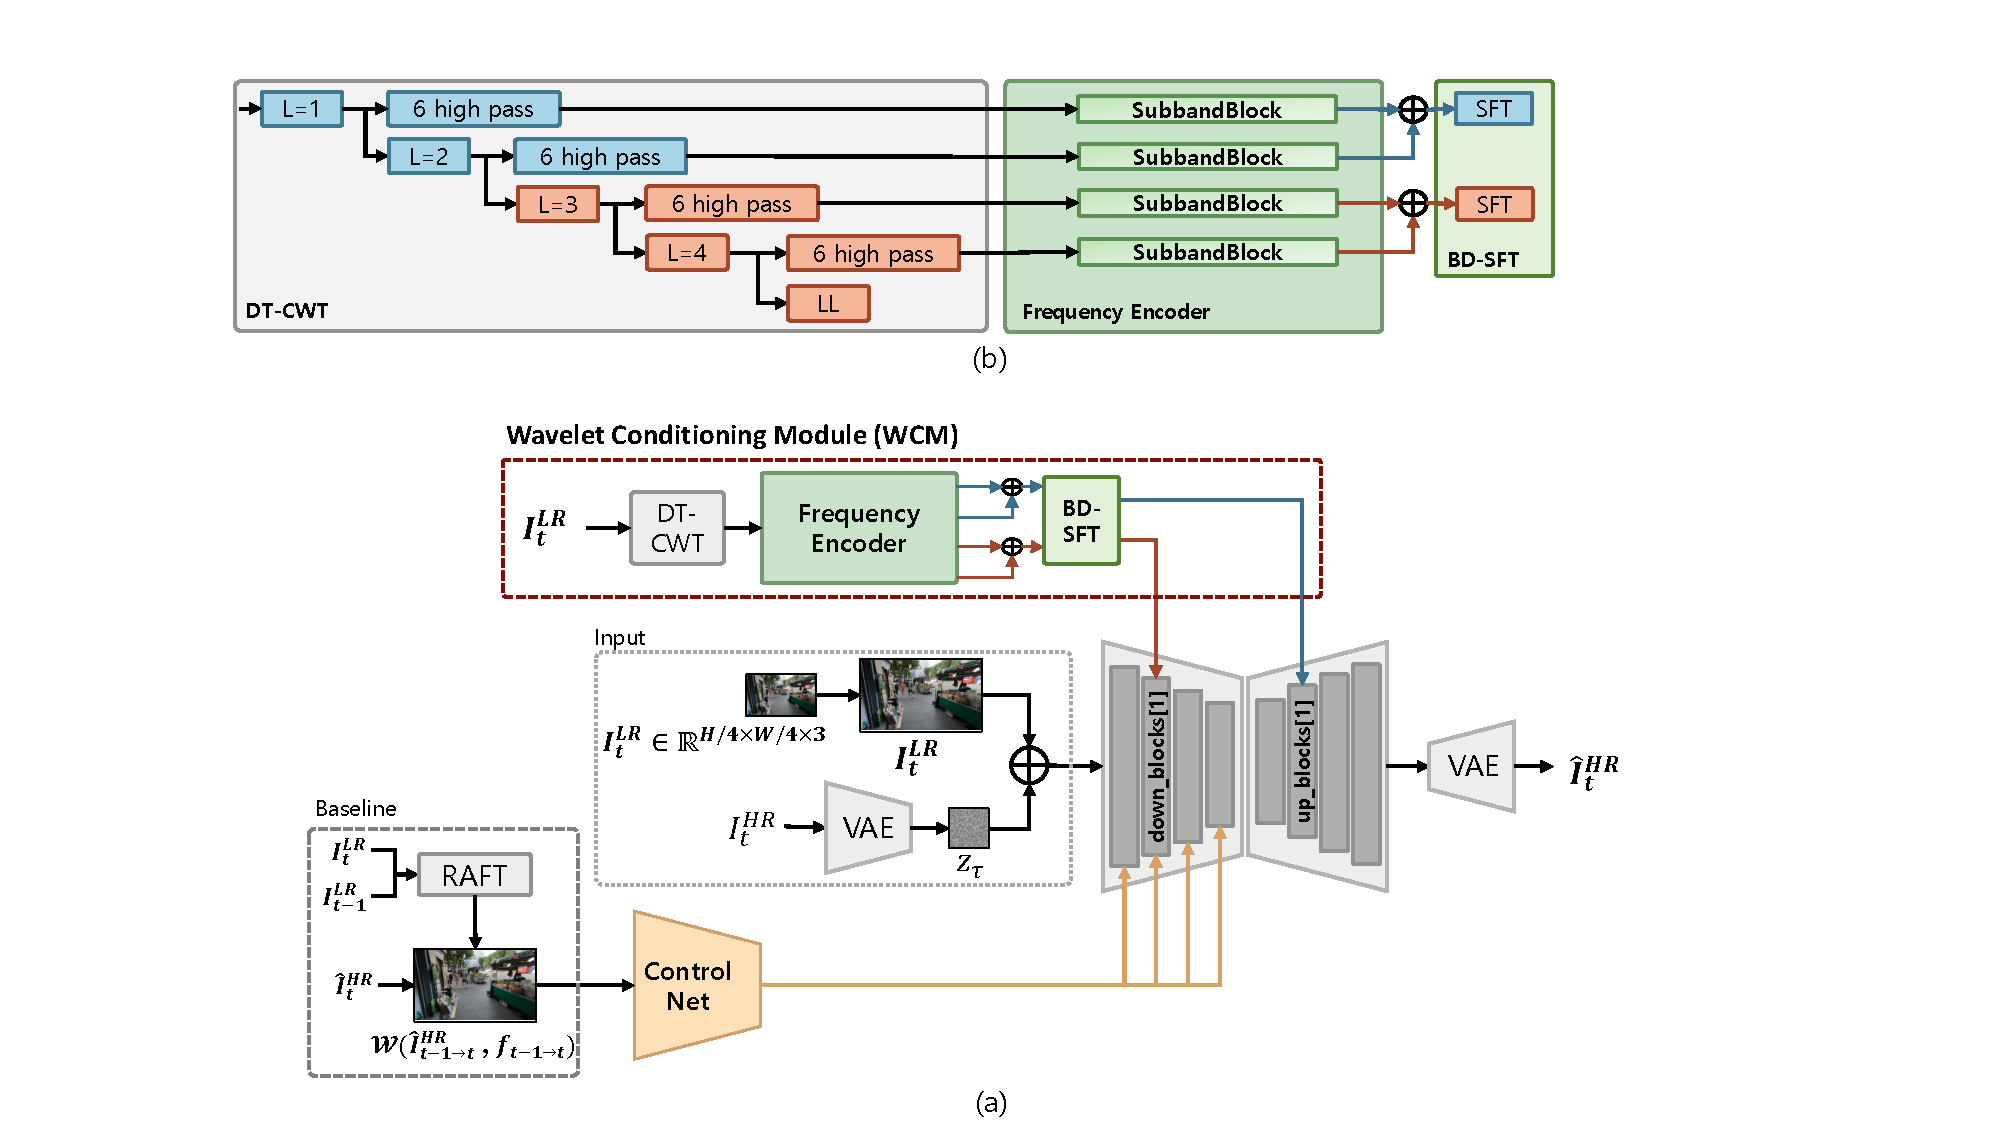
\includegraphics[
    width=\textwidth,
    trim={0 0 170 0},
    clip
]{fig/overall_architecture.pdf}
\caption{Overall architecture of the proposed framework. (a) The Wavelet Conditioning Module (WCM) consists of DT-CWT decomposition, the Frequency Encoder, and the BD-SFT injection: the high-frequency band is injected at the U-Net decoder (blue), and the low-frequency band is injected at the U-Net encoder (red). (b) The Frequency Encoder contains four SubbandBlocks, one per DT-CWT scale ($L{=}1,\ldots,4$). The remaining components, including the RAFT-based temporal warping, follow the StableVSR baseline.}
\label{fig:overall_architecture}
\end{figure}

\subsection{System Architecture}
\label{subsec:system_architecture}

The overall pipeline, illustrated in Figure~\ref{fig:overall_architecture}, 
operates in three stages within the WCM. First, a four-level 
($J=4$) DT-CWT decomposes the LR input $I^{LR}_t$ into multi-scale 
complex wavelet coefficients. Second, the Frequency Encoder 
processes these coefficients into two band-separated modulation 
tensors $(\gamma_\mathcal{H}, \beta_\mathcal{H})$ and 
$(\gamma_\mathcal{L}, \beta_\mathcal{L})$ via four SubbandBlocks. 
Third, the BD-SFT injects these tensors into the U-Net at 
\texttt{up\_blocks[1]} and \texttt{down\_blocks[1]}, respectively. 
Finally, the denoised latent is decoded back to the pixel space 
by the pre-trained VAE to produce $\hat{I}^{HR}_t$.

The pre-trained U-Net ($\sim$472M) and VAE ($\sim$55M) remain frozen 
to preserve their generative prior. Following the StableVSR 
baseline, the ControlNet ($\sim$208M) is jointly fine-tuned 
alongside the proposed Frequency Encoder ($\sim$6.22M). The 
Frequency Encoder constitutes the unique technical contribution of 
this work and adds only $\sim$3\% trainable parameters relative to 
the ControlNet baseline.


%==================== Section =====================%
\section{Frequency-Domain Conditioning via DT-CWT}
\label{sec:dtcwt_conditioning}

We adopt the DT-CWT~\cite{selesnick2005dtcwt} as the 
frequency-domain decomposition of the LR input. We choose DT-CWT 
over the standard discrete wavelet transform (DWT) and the Fourier 
transform for three reasons. First, DT-CWT exhibits 
\emph{near shift-invariance}, in contrast to the DWT which is 
sensitive to spatial translation~\cite{selesnick2005dtcwt}. Second, 
DT-CWT provides \emph{six directional subbands} per scale 
($\pm 15^\circ$, $\pm 45^\circ$, $\pm 75^\circ$), whereas the DWT 
only provides three (LH, HL, HH); this finer directional resolution 
is essential for capturing texture orientation in natural images. 
Third, DT-CWT yields \emph{complex-valued} coefficients with 
explicit phase information, enabling our magnitude-phase pathway 
separation. While the Fourier transform also provides phase, it 
lacks the spatial localization that wavelets offer, making it less 
suitable for spatially varying conditioning.

\begin{figure}[H]
\centering
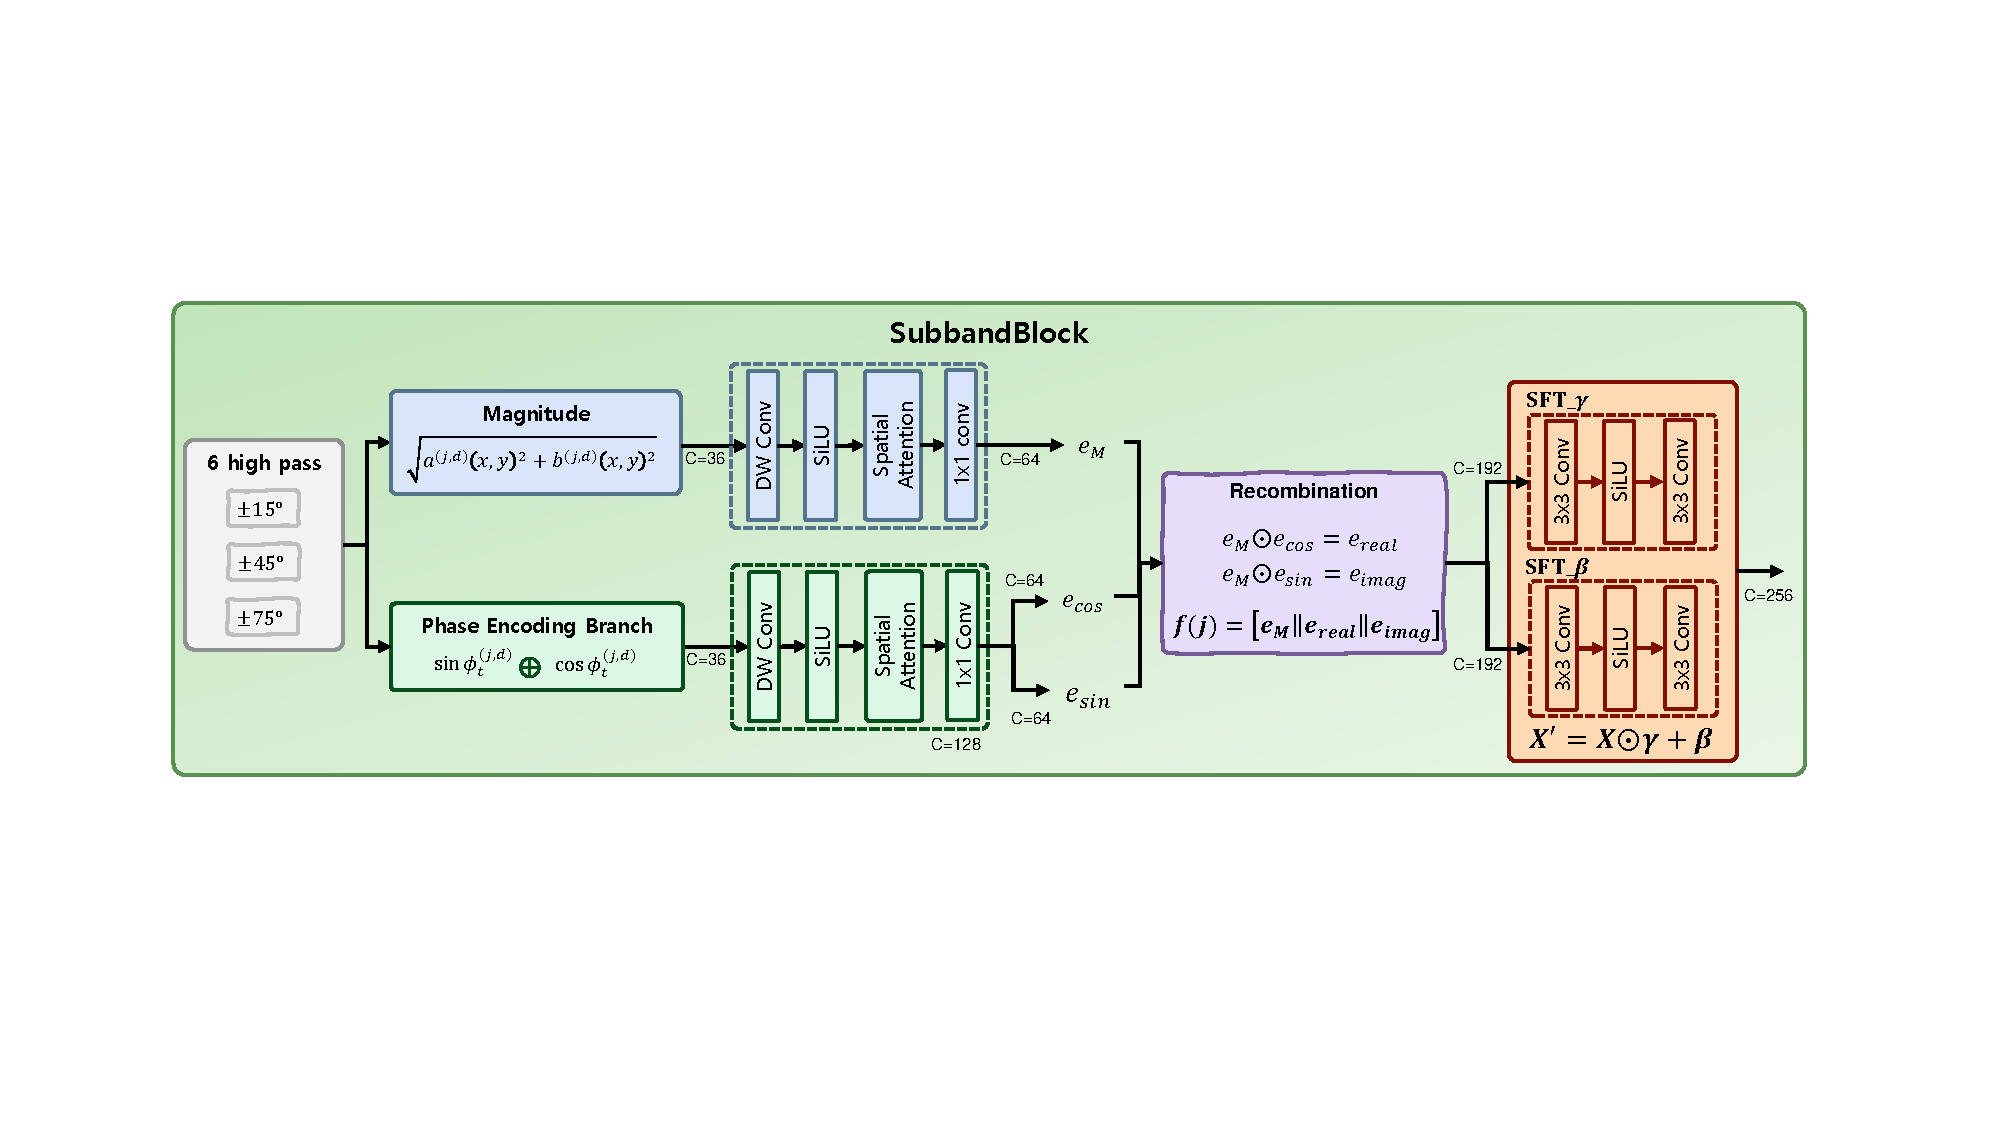
\includegraphics[
    width=\textwidth,
    trim={50 130 50 130},
    clip
]{fig/subbandblock.pdf}
\caption{Architecture of the proposed SubbandBlock. The six high-pass complex wavelet coefficients of a single DT-CWT scale are decomposed into Magnitude and Phase Encoding branches, recombined into complex-valued embeddings, and projected by SFT heads ($\mathrm{SFT}\_\gamma$, $\mathrm{SFT}\_\beta$) to produce the per-scale modulation parameters $\gamma^{(j)}, \beta^{(j)}$.}
\label{fig:subbandblock}
\end{figure}

\subsection{Multi-Scale Decomposition and Band Partitioning}
\label{subsec:dtcwt_decomposition}

Following the DT-CWT formulation of Selesnick et 
al.~\cite{selesnick2005dtcwt}, a four-level DT-CWT applied to 
$I^{LR}_t$ produces a real-valued lowpass component (LL) 
$I^{LP}_t$ and \emph{six high-pass} complex-valued coefficients 
$C^{(j,d)}_t \in \mathbb{C}^{H_{LR}/2^j \times W_{LR}/2^j \times 3}$ 
per scale:
\begin{equation}
    \mathrm{DTCWT}_{J=4}(I^{LR}_t) = 
    \big( I^{LP}_t,\, \{C^{(j,d)}_t\}_{j=1, d=1}^{4,\,6} \big),
    \label{eq:dtcwt_decomp}
\end{equation}
with six subbands per scale oriented at approximately $\pm 15^\circ$, 
$\pm 45^\circ$, $\pm 75^\circ$. Here, the directional index $d \in 
\{1, \ldots, 6\}$ indexes these six orientations, the scale index 
$j \in \{1, 2, 3, 4\}$ corresponds to the decomposition levels 
denoted $L{=}1, \ldots, L{=}4$ in 
Figure~\ref{fig:overall_architecture}(b), and $H_{LR}, W_{LR}$ 
denote the spatial dimensions of the LR input.

\paragraph{Choice of $J=4$.}
We use $J=4$ decomposition levels for three reasons: 
(i) four levels yield a balanced $2{:}2$ partition into HIGH 
($j=1, 2$) and LOW ($j=3, 4$) bands, ensuring equal expressiveness 
for both pathways; (ii) the spatial size of the $j=4$ subband, 
when computed from the LR input, becomes $H_{LR}/16 \times 
W_{LR}/16$. With the standard SD-VAE 8$\times$ downsampling and 
the U-Net's 2$\times$ downsampling at \texttt{down\_blocks[1]}, 
this resolution is compatible with our BD-SFT injection scheme 
without aggressive resampling; (iii) for typical SR targets, $J=4$ 
provides sufficient frequency resolution without truncating to 
overly small lowpass dimensions.

\paragraph{Band partitioning.}
The four scales are partitioned into two non-overlapping bands at 
the boundary between $j=2$ and $j=3$: $\mathcal{H} = \{j{=}1, 
j{=}2\}$ (covering normalized frequencies $[1/8, 1/2]$ 
cycles/pixel: fine textures, sharp edges) and $\mathcal{L} = 
\{j{=}3, j{=}4\}$ (covering $[0, 1/8]$ cycles/pixel: coarse 
structures). This partitioning is motivated by three 
considerations:
\begin{itemize}
    \item \textbf{Symmetric expressiveness.} The $2{:}2$ split 
    provides balanced channel capacity between the two 
    band-specialized SFT pathways, with each band contributing 
    $2 \times 256 = 512$ channels matching the U-Net's 
    \texttt{block\_out\_channels[1]}.
    \item \textbf{Spectral interpretation.} The boundary cleanly 
    separates the upper half of the LR signal spectrum (textural 
    detail) from the lower half (coarse structure), enabling 
    each SFT pathway to specialize on a non-overlapping frequency 
    range.
    \item \textbf{Architectural alignment.} The $j \ge 3$ levels 
    have spatial sizes ($\le H_{LR}/8$) that are easily upsampled 
    to the U-Net feature resolution, while the $j \le 2$ levels 
    require minimal resampling for high-resolution decoder 
    injection.
\end{itemize}
Each band is routed to a corresponding U-Net injection point in 
the BD-SFT scheme (Section~\ref{sec:bd_sft}).

\subsection{Magnitude and Phase Extraction}
\label{subsec:mag_phase_extraction}

Each complex coefficient $C^{(j,d)}_t = a^{(j,d)}_t(x,y) + 
j\,b^{(j,d)}_t(x,y)$, where $a, b$ denote the real and imaginary 
parts respectively, is characterized by its magnitude
\begin{equation}
    M^{(j,d)}_t(x,y) = |C^{(j,d)}_t(x,y)| = 
    \sqrt{a^{(j,d)}_t(x,y)^2 + b^{(j,d)}_t(x,y)^2}
    \label{eq:magnitude}
\end{equation}
and phase $\phi^{(j,d)}_t = \angle C^{(j,d)}_t \in [-\pi, \pi)$. 
Direct processing of the raw phase is problematic because of the 
$2\pi$-wraparound discontinuity. Following the principle of 
representing angular or periodic quantities via $(\sin, \cos)$ 
pairs as commonly used in positional 
encodings~\cite{vaswani2017attention,mildenhall2020nerf}, we adopt 
a trigonometric encoding that maps the phase onto the unit circle:
\begin{equation}
    \mathcal{T}(\phi^{(j,d)}_t) = 
    \big( \sin \phi^{(j,d)}_t,\; \cos \phi^{(j,d)}_t \big),
    \label{eq:trig_encoding}
\end{equation}
which is continuous across the $\pm \pi$ boundary and provides a 
normalized, bounded representation suitable as neural network 
input. We emphasize that $\mathcal{T}(\phi)$ is a 
two-dimensional \emph{encoding} of the scalar phase, not the phase 
itself; the original phase $\phi$ remains a scalar quantity used 
in the loss function (Section~\ref{subsec:wavelet_loss}). In 
practice, the encoding is computed directly without explicit 
arctangent operation as
\begin{equation}
    \cos\phi^{(j,d)}_t = \frac{a^{(j,d)}_t}
    {M^{(j,d)}_t + \epsilon}, \quad
    \sin\phi^{(j,d)}_t = \frac{b^{(j,d)}_t}
    {M^{(j,d)}_t + \epsilon},
    \label{eq:trig_encoding_compute}
\end{equation}
with $\epsilon = 10^{-8}$ to avoid division by zero.

%==================== Section =====================%
\section{Frequency Encoder}
\label{sec:freq_encoder}

The Frequency Encoder transforms the DT-CWT coefficients into 
U-Net-compatible modulation parameters $(\gamma, \beta)$. As shown 
in Figure~\ref{fig:overall_architecture}(b), it consists of four 
SubbandBlock modules---one per DT-CWT scale ($L{=}1, \ldots, 4$)
---whose outputs are grouped into the high- and low-frequency 
band representations defined in Section~\ref{subsec:dtcwt_decomposition}.

\subsection{SubbandBlock}
\label{subsec:subband_block}

Each SubbandBlock processes the six high-pass complex coefficients 
of a single DT-CWT scale through three stages: a Magnitude branch 
and a Phase Encoding Branch operating in parallel, a Recombination 
stage, and SFT-head generation ($\mathrm{SFT}\_\gamma$, 
$\mathrm{SFT}\_\beta$). Both branches apply the same operator 
sequence $\mathcal{E}(\cdot) = \mathrm{Conv}_{1\times1} \circ 
\mathrm{SA} \circ \mathrm{SiLU} \circ \mathrm{DWConv}_{3\times3}$, 
where $\mathrm{SA}(\cdot)$ denotes a CBAM-style spatial 
attention~\cite{woo2018cbam} chosen to emphasize the directional 
structure inherent to the wavelet subbands. With six directional 
subbands per scale and three RGB channels, each branch input has 
$C{=}36$ channels:
\begin{equation}
    e_M^{(j)} = \mathcal{E}(M^{(j)}) \in 
    \mathbb{R}^{C_m \times H_j \times W_j}, 
    \quad 
    e_\phi^{(j)} = \mathcal{E}(\mathcal{T}(\phi^{(j)})) \in 
    \mathbb{R}^{2C_m \times H_j \times W_j},
    \label{eq:branches}
\end{equation}
with $C_m = 64$. We refer to $e_M^{(j)}$ as the Magnitude branch 
output and $e_\phi^{(j)}$ as the Phase Encoding Branch output, 
where the latter operates on the trigonometric encoding 
$\mathcal{T}(\phi)$ rather than the scalar phase. In the 
Recombination stage, the phase output is split along the channel 
dimension into $(e_{\sin}^{(j)}, e_{\cos}^{(j)})$, then recombined 
with the magnitude into complex-valued embeddings:
\begin{equation}
    e_{\mathrm{real}}^{(j)} = e_M^{(j)} \odot e_{\cos}^{(j)}, \quad
    e_{\mathrm{imag}}^{(j)} = e_M^{(j)} \odot e_{\sin}^{(j)},
    \label{eq:recombination}
\end{equation}
mirroring the polar-to-Cartesian relation 
$Re^{i\phi} = R\cos\phi + iR\sin\phi$ in the embedding space. 
The final feature is the channel-wise concatenation
\begin{equation}
    f^{(j)} = [e_M^{(j)} \,\|\, e_{\mathrm{real}}^{(j)} \,\|\, 
    e_{\mathrm{imag}}^{(j)}] \in \mathbb{R}^{3C_m \times H_j \times W_j},
    \label{eq:concat_features}
\end{equation}
yielding a 192-channel feature map ($3 \times 64$). This is fed 
into two SFT heads, $\mathrm{SFT}\_\gamma$ and 
$\mathrm{SFT}\_\beta$, each consisting of $\mathrm{Conv}_{3\times3} 
\to \mathrm{SiLU} \to \mathrm{Conv}_{3\times3}$, producing 
per-scale modulation parameters $\gamma^{(j)}$ and $\beta^{(j)}$ 
with 256 output channels each. To preserve the pre-trained U-Net's 
behavior at the start of training, the second convolution of each 
SFT head is zero-initialized in weight, with bias set to $1$ for 
$\gamma$ and $0$ for $\beta$.

\subsection{Frequency-Separated Grouping}
\label{subsec:multi_level_grouping}

Per-scale outputs from the four SubbandBlocks are grouped into the 
two frequency bands. Within each group, the two scales are 
spatially aligned via bilinear interpolation and concatenated 
along the channel dimension:
\begin{align}
    \gamma_\mathcal{H} &= [\gamma^{(1)} \,\|\, \gamma^{(2)}], 
    \quad 
    \beta_\mathcal{H} = [\beta^{(1)} \,\|\, \beta^{(2)}], 
    \label{eq:high_concat}\\
    \gamma_\mathcal{L} &= [\gamma^{(3)} \,\|\, \gamma^{(4)}], 
    \quad 
    \beta_\mathcal{L} = [\beta^{(3)} \,\|\, \beta^{(4)}].
    \label{eq:low_concat}
\end{align}
Concatenation, rather than weighted summation, preserves the distinct 
information of each scale. The resulting modulation tensors have 
$2 \times 256 = 512$ channels, exactly matching the U-Net's 
\texttt{block\_out\_channels[1]}.

\subsection{Parameter Analysis}
\label{subsec:param_analysis}

Each SubbandBlock consists of a Magnitude branch, a Phase Encoding 
Branch, and two SFT heads, all built from lightweight convolutional 
operations. The mid-channel dimension is set to $C_m = 64$, 
following standard practice in lightweight conditioning encoders. 
With four SubbandBlocks, the total trainable parameter count of 
the Frequency Encoder is $\sim$6.22M, corresponding to only 
$\sim$3\% additional parameters relative to the $\sim$208M 
ControlNet baseline, demonstrating that the proposed 
wavelet-conditioned BD-SFT modulation is parameter-efficient.


%==================== Section =====================%
\section{Band-Decoupled SFT Injection into U-Net}
\label{sec:bd_sft}

The two band-specialized modulation tensors generated by the 
Frequency Encoder are injected into the diffusion U-Net at 
functionally distinct stages, modulating intermediate features via 
spatial feature transform (SFT)~\cite{wang2018sft}. We refer to 
this scheme as the \emph{Band-Decoupled SFT} (BD-SFT), reflecting 
the frequency-domain separation of the modulation pathways into 
asymmetric U-Net injection points.

\subsection{Spatial Feature Transform Modulation}
\label{subsec:sft_modulation}

At each injection point, the corresponding intermediate feature map 
$X \in \mathbb{R}^{C \times h \times w}$ is modulated via spatial 
feature transform~\cite{wang2018sft}:
\begin{equation}
    X' = X \odot \gamma + \beta,
    \label{eq:sft_modulation}
\end{equation}
where $\gamma$ and $\beta$ are spatially aligned modulation 
parameters generated by the Frequency Encoder. SFT was originally 
introduced for image super-resolution to inject semantic priors 
into a generative network~\cite{wang2018sft}; we adopt it here to 
inject frequency-domain conditioning, leveraging its proven 
effectiveness in feature-wise modulation. Compared to alternative 
conditioning mechanisms such as cross-attention (quadratic 
complexity in spatial size) or AdaIN (globally uniform modulation), 
SFT provides spatially varying affine transformation at low 
computational cost, which is well-suited to our spatially-localized 
wavelet conditioning.

\subsection{Asymmetric Injection Points}
\label{subsec:injection_points}

We inject the LOW-band SFT at \texttt{down\_blocks[1]} (encoder) 
and the HIGH-band SFT at \texttt{up\_blocks[1]} (decoder), based 
on three considerations:
\begin{itemize}
    \item \textbf{Architectural alignment.} Both blocks have 
    \texttt{block\_out\_channels[1]} $= 512$ channels, which 
    exactly matches the Frequency Encoder output 
    $\gamma, \beta \in \mathbb{R}^{512 \times h \times w}$. 
    Other U-Net blocks would require additional channel projection.
    
    \item \textbf{Functional separation.} Recent analyses of 
    diffusion U-Nets~\cite{si2024freeu,choi2022p2} have shown 
    that the encoder backbone progressively suppresses 
    high-frequency content while consolidating coarse structural 
    features, whereas the decoder reintroduces high-frequency 
    details through upsampling and skip-connection fusion. Our 
    injection scheme aligns with this observation: LOW-band 
    guidance reinforces the encoder's structural abstraction, 
    while HIGH-band guidance augments the decoder's detail 
    synthesis at the stage where it has the most direct impact 
    on the output.
    
    \item \textbf{Conservative design.} A single injection per 
    band keeps parameter overhead low and preserves the clean 
    identity initialization across both injection points.
\end{itemize}
The modulation tensors are spatially aligned to $(h, w)$ via 
bilinear interpolation if needed; the channel dimension $C = 512$ 
is matched by construction.



%==================== Section =====================%
\section{Training Loss}
\label{sec:training_objective}

In addition to the standard $\epsilon$-prediction MSE loss 
$\mathcal{L}_{\mathrm{MSE}}$ of latent diffusion 
models~\cite{ho2020ddpm,rombach2022ldm}, we apply a band-decoupled 
wavelet loss in the RGB pixel space to explicitly supervise the 
frequency content of the reconstructed HR image.

\subsection{Band-Decoupled Wavelet Loss}
\label{subsec:wavelet_loss}

The denoised latent is decoded by the VAE to obtain the predicted HR 
image $\hat{I}^{HR}_t$, and DT-CWT decomposition is applied to both 
$\hat{I}^{HR}_t$ and the ground truth $I^{HR}_t$. The wavelet loss 
is decomposed across frequency bands as
\begin{equation}
    \mathcal{L}_{\mathrm{wav}} 
    = \lambda_\mathcal{H} \!\sum_{j \in \mathcal{H}} \!
    \big\| |\hat{C}^{(j)}_t| - |C^{(j)}_t| \big\|_1
    + \lambda_\mathcal{L} \!\sum_{j \in \mathcal{L}} \!
    \mathcal{L}_j^{\mathrm{mp}}
    + \lambda_{\mathrm{LP}} \big\| \hat{I}^{LP}_t - I^{LP}_t \big\|_1,
    \label{eq:wav_loss}
\end{equation}
where the per-level magnitude-phase term for the low-frequency band 
is defined as
\begin{equation}
    \mathcal{L}_j^{\mathrm{mp}} = 
    \big\| |\hat{C}^{(j)}_t| - |C^{(j)}_t| \big\|_1 
    + \mathbb{E}\!\left[ |C^{(j)}_t| 
    \big(1 - \cos(\hat{\phi}^{(j)}_t - \phi^{(j)}_t)\big) \right].
    \label{eq:low_mp_loss}
\end{equation}
We propose this magnitude-weighted angular distance term to 
supervise the structural integrity of the low-frequency band. The 
cosine-based phase term $1 - \cos(\Delta\phi) \in [0, 2]$ is the 
standard angular distance in directional 
statistics~\cite{mardia2009directional} and is wraparound-safe by 
construction. The ground-truth magnitude $|C^{(j)}_t|$ acts as an 
importance weight, so phase mismatch in regions with significant 
low-frequency energy (e.g., strong structural edges) is penalized 
more heavily, while flat regions with negligible magnitude 
contribute little. Magnitude-aware weighting of phase errors is 
conceptually aligned with phase-aware spectral losses in audio 
processing~\cite{choi2019phaseaware}, where phase fidelity is 
prioritized in high-energy regions.

\paragraph{Asymmetric supervision.}
The high-frequency band is supervised in magnitude only, allowing 
the network to freely synthesize textural details without the 
constraint of exact phase matching. The low-frequency band 
additionally constrains phase, reflecting the structural importance 
of low-frequency phase information.

\paragraph{Loss weights.}
We set the loss weights to $\lambda_\mathcal{H} = 0.1$, 
$\lambda_\mathcal{L} = 1.0$, and $\lambda_{\mathrm{LP}} = 1.0$ 
based on the design intent that the high-frequency band acts as a 
soft texture prior---encouraging detail synthesis without strictly 
enforcing exact magnitude matching---while the low-frequency band 
requires precise structural matching including phase. The smaller 
$\lambda_\mathcal{H}$ also balances the gradient magnitudes from 
the two bands during training. These specific values were adopted 
as initial settings consistent with this design intent.

\subsection{Total Loss}
\label{subsec:combined_loss}

The total training objective is
\begin{equation}
    \mathcal{L}_{\mathrm{total}} = \mathcal{L}_{\mathrm{MSE}} 
    + \lambda_{\mathrm{wav}} \cdot 
    \mathbb{1}_{[t_{\mathrm{step}} \bmod K = 0]} \cdot 
    \mathcal{L}_{\mathrm{wav}},
    \label{eq:total_loss}
\end{equation}
with $\lambda_{\mathrm{wav}} = 1.0$ and $K = 4$. The wavelet loss 
is applied only every $K$ optimization steps because evaluating 
$\mathcal{L}_{\mathrm{wav}}$ requires VAE-decoding the predicted 
latent into the pixel space, which is computationally expensive. 
We adopt $K = 4$ as a practical compromise to limit the 
VAE-decoding overhead while still providing regular 
frequency-domain supervision throughout training.